\documentclass[a4paper,12pt]{book}
\usepackage{graphicx}
\usepackage[export]{adjustbox}
\usepackage{subcaption}
\graphicspath{{Pics/}}
\usepackage{charter}
\usepackage{fancyhdr}
\usepackage{enumerate}
\usepackage{enumitem}
\usepackage{siunitx}
\usepackage{amssymb}
\usepackage{longtable}
\usepackage{multicol}
\usepackage{multirow}
\usepackage{hhline}
\usepackage{parskip}
\setlength{\parskip}{6pt}
\usepackage{ragged2e}
\usepackage{geometry} %margin
\geometry{left=2.1cm,right=2.1cm,top=3cm,bottom=3cm}
\usepackage{setspace}
\SetSinglespace{1.2}
\singlespacing
\renewcommand{\ttfamily}{\fontfamily{pcr}\selectfont}
%\renewcommand{\familydefault}{\rmdefault}

\usepackage[,table]{xcolor}
\definecolor{LightBlue}{cmyk}{0.16,0.03,0.04,0}
\definecolor{Title}{cmyk}{0.8,0.1,0,0.3}
\setlength{\arrayrulewidth}{0.3mm}
\setlength{\tabcolsep}{2pt}
\setlength{\headheight}{15pt}
\renewcommand{\arraystretch}{1}
\usepackage{tikz}
\usepackage{nicematrix}
\newcommand*\circled[1]{\tikz[baseline=(char.base)]{\node[shape=circle,draw,inner sep=1pt] (char) {#1};}}

\newcolumntype{s}{>{\columncolor{Title}\RaggedLeft} m{3.5em}} % columntype for chapter title
\newcolumntype{d}{>{\columncolor{LightBlue}\RaggedRight} m{\textwidth}} % columntype for code bloc
\newcolumntype{a}{>{\columncolor{LightBlue}\RaggedRight} m{0.96\textwidth}} % columntype for secondary code bloc

\usepackage{titlesec}
\usepackage[hidelinks]{hyperref}
\urlstyle{same}

\captionsetup[figure]{labelsep=period,font={bf}}
\captionsetup[table]{font={bf},labelsep=period}

\newcommand{\titlename}{}

\newcommand{\chaptertitle}[2]{ %reset chapter format
\vspace{-120pt}
\gdef\titlename{#1}
{
\SetSinglespace{1.1}
\singlespacing
\Huge\bfseries
\setlength{\tabcolsep}{8pt}
\renewcommand{\arraystretch}{1.5}
\begin{tabular}{s >{\RaggedRight}m{14.5em}}
\textcolor{white}{Chapter\newline\thechapter}&\textcolor{Title}{#2}
\end{tabular}
}
}

\newcommand{\partpic}[1]{%insert picture
    \tikz[remember picture,overlay] \node at (current page.center){\includegraphics[width=\paperwidth]{#1}};
}

\titleformat{\part} %reset part %format
{\huge\bfseries} % format
{} % label
{0em} % sep
{\Centering} % before-code

\titleformat{\chapter} %reset chapter %format
{\huge\bfseries} % format
{} % label
{0em} % sep
{\Centering} % before-code
\titlespacing{\chapter}{0pt}{0pt}{0pt}

\titleformat{\section} %reset section %format
{\Large\bfseries} % format
{\textcolor{Title}{\thesection}} % label
{0.5em} % sep
{\color{Title}} % before-code
\titlespacing{\section}{0pt}{12pt}{6pt}

\titleformat{\subsection} %reset subsection %format
{\large\bfseries} % format
{\textcolor{Title}{\thesubsection}} % label
{0.5em} % sep
{\color{Title}} % before-code
\titlespacing{\subsection}{0pt}{8pt}{6pt}

\newenvironment{term}[1]{
    \textbf{#1}

    \leftskip 1em
    \parskip 0pt
}

\newenvironment{secterm}[1]{
    \textbf{#1}

    \leftskip 2em
    \parskip 0pt
}

\newenvironment{codebloc}{ %define code bloc style
    \ttfamily\footnotesize
    \renewcommand{\arraystretch}{1}
}

\newcommand{\note}[2][NOTE]{ %Note/Tips
\vspace{6pt}
\begin{tabular}{b{\textwidth}}
\hline
\fontfamily{phv}\selectfont \textbf{#1}\\
\leftskip 1em #2\\
\hline
\end{tabular}
}

\newcommand{\secnote}[2][NOTE]{ %Note/Tips
\vspace{6pt}
\begin{tabular}{b{0.93\textwidth}}
\hline
\fontfamily{phv}\selectfont \textbf{#1}\\
\leftskip 1em #2\\
\hline
\end{tabular}
}

\title{ESP32-C3 Wireless Adventure\par \Large A comprehensive guide to IoT}
\author{Espressif Systems}
\date{\today}

\pagestyle{fancy} % reset head&foot
\fancyhead{} % clear all header fields
\renewcommand\headrulewidth{0pt}
\fancyfoot{} % clear all footer fields
\setcounter{chapter}{11}

\begin{document}

\fancyfoot[LE]{\fontfamily{cmss}\selectfont{\textbf{\thepage} \ \textit{ESP32-C3 Wireless Adventure: A comprehensive guide to IoT}}}
\fancyfoot[RO]{\fontfamily{cmss}\selectfont{\textit{Chapter \thechapter. \titlename} \ \textbf{\thepage}}}

{\makeatletter
\let\ps@plain\ps@empty
\makeatother
\part[Optimisation and Mass Production]{\partpic{Starting/4c}}
}

\chapter[Power Management and Low-Power Optimisation]{\chaptertitle{Power Management and Low-Power Optimisation}{Power Management and\newline Low-Power Optimisation}}

\vspace{36pt}
With the wide application of IoT products, people can see more and more IoT products in daily life, such as smart watches, smart sockets, smart light bulbs, smart speakers, etc. Many of these IoT products are under pressure to reduce their power consumption because they are powered by battery or require certification for energy consumption. For example, the CEC Tile 20 specification mandates that smart bulbs must not exceed a standby power consumption of 0.2W to obtain energy consumption certification in California, USA. Battery-powered smartwatches also aim to extend their working hours. Developers of such IoT products must prioritise power consumption as a crucial consideration during product development. They must have a comprehensive understanding of the power consumption characteristics of the chips they use, and be skilled in utilising the relevant chips in practical IoT projects. To achieve this, they should prioritise using low-power wireless communication technologies, such as Bluetooth LE, and employ low-power circuit design in their implementations. This ensures that power consumption is minimised throughout the development process.

In low-power scenarios, the lifetime of a battery-powered device and its ability to pass energy certification are often determined by its average current. This average current is influenced by several factors, including the current in different low-power modes, the operating current in active states, the duration of low-power mode activation or deactivation, and the processing power of the CPU. ESP32-C3 provides chip-level support for low-power scenarios. It employs advanced power management technology to switch between different power modes and features intelligent low-power peripherals that help reduce CPU wakeup times, resulting in further reduction of overall power consumption.

\section{ESP32-C3 Power Management}
Power management algorithm included in ESP-IDF can adjust the advanced peripheral bus (APB) frequency, CPU frequency, and put the chip into Light-sleep mode to run an application at smallest possible power consumption, given the requirements of application components. Additionally, the chip automatically enters Light-sleep mode when idle, reducing the power consumption during application runs. The ESP32-C3's various low-power modes are discussed in detail in Section 12.2. Enabling power management features comes at the cost of increased interrupt latency. Extra latency depends on several factors, such as the CPU frequency, single/dual core mode, whether frequency switch is required.

Applications can acquire/release locks to control the power management algorithm. When an application acquires a lock, the operation of power management algorithm is restricted. When the lock is released, such restrictions are removed. Power management locks have acquire/release counters. If the lock has been acquired a number of times, it needs to be released the same number of times to remove associated restrictions.

ESP32-C3 supports three types of locks described in Table 12.1.

\begin{table}[h!]
    \renewcommand{\arraystretch}{1.2}
    \caption{Power management locks}
    \begin{tabular}{|>{\footnotesize}m{0.32\textwidth}|>{\footnotesize}m{0.66\textwidth}|}
        \hline
        \rowcolor{LightBlue}\multicolumn{1}{|c|}{\textbf{Power management lock}}&\multicolumn{1}{c|}{\textbf{Description}}\\
        \hline
        \verb|SP_PM_CPU_FREQ_MAX|&Requests CPU frequency to be at the maximum value set with \verb|esp_pm_configure()|. For ESP32-C3, this value can be set to 80 MHz, 160 MHz, or 240 MHz.\\
        \hline
        \verb|ESP_PM_APB_FREQ_MAX|&Requests the APB frequency to be at the maximum supported value. For ESP32-C3, this is 80 MHz.\\
        \hline
        \verb|ESP_PM_NO_LIGHT_SLEEP|&Disable automatic switching to Light-sleep mode\\
        \hline
    \end{tabular}
\end{table}

Applications can acquire or release power management locks in a way that can accommodate scenarios where power management is not required. For example, driver for a peripheral clocked from APB can request the APB frequency to be set to 80 MHz while the peripheral is used; RTOS can request the CPU to run at the highest configured frequency while there are tasks ready to run; A peripheral driver may need interrupts to be enabled, which means it will have to request disabling Light-sleep mode.

Since requesting higher APB or CPU frequencies or disabling Light-sleep mode causes higher current consumption, please keep the usage of power management locks by components to a minimum.

\subsection{Dynamic Frequency Scaling}
When power management is enabled, the peripheral bus (APB) frequency and CPU frequency may change during operation. This process is called Dynamic Frequency Scaling (DFS). When DFS is enabled, the APB frequency can be changed multiple times within a single RTOS tick. The APB frequency change does not affect the operation of some peripherals, while other peripherals may have issues. For example, Timer Group peripheral timers will keep counting, however, the speed at which they count will change proportionally to the APB frequency. Therefore, developers should understand which peripherals will be affected by DFS and which peripherals will not. With the continuous improvement of ESP-IDF development, more and more peripheral drivers will not be affected by DFS.

The following peripherals are not affected by DFS when clocked from a specific clock source:

\begin{itemize}
    \item \textbf{UART}: If \verb|REF_TICK| is used as the clock source, UART is not affected by DFS. Otherwise, it will be affected by DFS.
    \item \textbf{LEDC}: If \verb|REF_TICK| is used as the clock source, LEDC is not affected by DFS. Otherwise, it will be affected by DFS.
    \item \textbf{RMT}: If \verb|REF_TICK| or XTAL is used as the clock source, RMT is not affected by DFS.
\end{itemize}

Currently, the following peripheral drivers are not affected by DFS. These drivers will acquire the \verb|ESP_PM_APB_FREQ_MAX| lock for the duration of the transaction and release the lock upon the completion of the the transaction automatically.

\begin{itemize}
    \item \textbf{SPI host}
    \item \textbf{I2C}
    \item \textbf{I2S} (if an APLL clock is used, I2S acquires \verb|ESP_PM_NO_LIGHT_SLEEP| power management lock.)
    \item \textbf{SPI slave}: between calls to \verb|spi_slave_initialize()| and \verb|spi_slave_free()|, SPI slave is not affected by DFS.
    \item \textbf{Wi-Fi}: between calls to \verb|esp_wifi_start()| and \verb|esp_wifi_stop()|, Wi-Fi is not affected by DFS. In Modem-sleep mode, when Wi-Fi is enabled, the chip releases the \verb|ESP_PM_APB_FREQ_MAX| power management lock upon turning off the RF module.
    \item \textbf{TWAI}: between calls to \verb|twai_driver_install()| and \verb|twai_driver_uninstall|\\ \verb|()|, TWAI is not affected by DFS.
    \item \textbf{Bluetooth}: between calls to \verb|esp_bt_controller_enable()| and \verb|esp_bt_con|\\ \verb|troller_disable()|, Bluetooth is not affected by DFS. In Modem-sleep mode, when Bluetooth is enabled, the chip releases \verb|ESP_PM_APB_FREQ_MAX| power management lock upon turning off the RF module, but still holds the \verb|ESP_PM_NO_LIGHT_SLEEP| power management lock unless \verb|CONFIG_BTDM_CTRL_LOW_POWER_CLOCK| is configured to the 32 kHz external crystal oscillator.
\end{itemize}

The following peripheral drivers are affected by DFS, so applications need to acquire or release locks themselves.

\begin{itemize}
    \item  PCNT
    \item Sigma-delta
    \item Timer Group
\end{itemize}

\subsection{Power Management Configuration}
Generally, automatic Light-sleep mode is used in conjunction with Modem-sleep mode and power management features, and the detailed configuration about how to enable automatic Light-sleep mode is described in Section 12.2.2.

\section{ESP32-C3 Low-Power Mode}
ESP32-C3 has an advanced Power Management Unit (PMU), which can flexibly power up different power domains of the chip, to achieve the best balance among chip performance, power consumption, and wakeup latency. ESP32-C3 features four predefined power modes that not only enable developers to fulfill the requirements of various IoT application scenarios but also pass rigorous power consumption certification tests. These power modes have been successfully utilised in numerous IoT projects, including smart lighting. ESP32-C3 offers an array of low-power solutions for these power modes, which can serve as a reference for developers to select and configure based on their specific requirements. The four power modes are as follows:

\begin{itemize}
    \item \textbf{Active mode}: The CPU and chip RF are powered on. The chip can receive, transmit, or listen.
    \item \textbf{Modem-sleep mode}: The CPU is operational, and the clock speed can be reduced. Wi-Fi base band, Bluetooth LE base band, and RF are disabled, but Wi-Fi and Bluetooth LE connection can remain active.
    \item \textbf{Light-sleep mode}: The CPU is paused. Wi-Fi base band, Bluetooth LE base band, and RF are disabled. Any wakeup events (MAC, host, RTC timer, or external interrupts) will wake up the chip. In automatic Light-sleep mode, Wi-Fi or Bluetooth LE can remain connected.
    \item \textbf{Deep-sleep mode}: CPU and most peripherals are powered down. Only the RTC memory and RTC peripherals are powered on. Wi-Fi base band, Bluetooth LE base band, and RF module are disabled.
\end{itemize}

By default, ESP32-C3 will enter Active mode after reset. In Active mode, all parts of ESP32-C3 work properly. When the CPU is not needed to operate continuously, such as when waiting for external activity to wake up, the chip can enter one of the low-power modes. Developers can select various power modes based on specific power consumption, wakeup delay, and available wakeup source requirements. With the exception of the Active mode, the other three modes are low-power modes. Table 12.2 lists the differences between the three low-power modes.

\begin{table}[h!]
    \renewcommand{\arraystretch}{1.2}
    \caption{Differences between the three low-power modes}
    \begin{NiceTabular}{|>{\Centering}m{11em}|>{\Centering}m{6.5em}|>{\Centering}m{5.5em}|>{\Centering}m{6.5em}|>{\Centering}m{6.5em}|}[hvlines]
    \CodeBefore
       \rowcolor{LightBlue}{1,2}
    \Body
    \Block{2-1}{\textbf{Part}}&\Block{2-1}{\textbf{Modem-sleep}}&\Block{1-2}{\textbf{Light-sleep}}&&\Block{2-1}{\textbf{Deep-sleep}}\\
    &&Automatic&Compulsory&\\
    Wi-Fi connection and Bluetooth LE connection&Remain&Remain&Disconnected&Disconnected\\
    GPIO&Remain&\Block{1-2}{Remain}&&Remain\\
    Wi-Fi&Off&\Block{1-2}{Off}&&Off\\
    System clock&On&\Block{1-2}{Off}&&Off\\
    RTC&On&\Block{1-2}{On}&&On\\
    CPU&On&\Block{1-2}{Paused}&&Off\\
    \end{NiceTabular}
\end{table}

\subsection{Modem-sleep mode}
Currently, Modem-sleep mode on ESP32-C3 is only applicable when Wi-Fi Station connection and Bluetooth LE connection are active. The mode takes effect after the Wi-Fi Station connection router and Bluetooth LE are connected, and the chip periodically switches between Active mode and Modem-sleep mode. In Modem-sleep mode, the baseband of Wi-Fi and Bluetooth LE is clock gated or turned off. When the RF module is turned off, ESP32-C3 can be automatically woken up without any delay (also, this can be done without configuring any wakeup source). After waking up from Modem-sleep mode, the chip’s RF module switches from Modem-sleep mode to Active mode, causing an increase in power consumption.

ESP32-C3 uses the Wi-Fi Delivery Traffic Indication Message (DTIM) beacon mechanism to maintain a connection to the router. In Modem-sleep mode, ESP32-C3 will power off the RF module between two DTIM beacons to save power, and automatically wake up the RF module just before the next DTIM beacon arrives. The duration of sleep is determined by the router’s DTIM beacon interval and the \verb|listen_interval| parameter of ESP32-C3. In Modem-sleep mode, ESP32-C3 remains connected to the Wi-Fi router, which allows it to receive interactive information from a smartphone or server through the router.

DTIM can usually indicate the frequency of data transmission when using a router. Typically, the DTIM beacon interval of a router ranges from 100 to 1000 ms.

ESP32-C3 uses the Bluetooth LE Connection Event to maintain a connection with the peer device. In Modem-sleep mode, ESP32-C3 will power off the RF module between the two Connection Events to save power, and automatically wakes up before the next Connection Event arrives, and the duration of sleep is determined by the Bluetooth LE connection parameters.

Modem-sleep mode is typically used in low-power applications where the CPU is required to work constantly and a Wi-Fi or Bluetooth LE connection must be maintained. For example, when using the ESP32-C3 in local voice wakeup applications, the CPU constantly collects and processes audio data.

\textbf{1. Wi-Fi Modem-sleep mode}

In development, users can use \verb|esp_wifi_set_ps()| function to set current Wi-Fi power save \verb|type|:

\begin{itemize}[leftmargin=1em]
    \item \verb|WIFI_PS_NONE|: not using Modem-sleep mode.
    \item \verb|WIFI_PS_MIN_MODEM|: ESP32-C3 wakes up to receive beacon every router DTIM beacon, i.e. 1 router interval.
    \item \verb|WIFI_PS_MAX_MODEM|: ESP32-C3 wakes up periodically to receive beacon. The interval can be configured via the \verb|listen_interval| parameter in \verb|wifi_sta_config_t| (unit: in units of the interval time of the router DTIM beacon). The default value is 3, which indicates an interval of 3 router beacons. The code is as follows:
\end{itemize}

\begin{codebloc}
\begin{tabular}{d}
\vspace{2pt}
\begin{verbatim}
1.  typedef enum {
2.      WIFI_PS_NONE,        /*< No power save*/
3.      WIFI_PS_MIN_MODEM,   /*< Minimum modem power saving. In this mode,
4.                station wakes up to receive beacon every DTIM period*/
5.      WIFI_PS_MAX_MODEM,   /*< Maximum modem power saving. In this mode,
6.                           interval to receive beacons is determined by the
7.                           listen_interval parameter in wifi_sta_config_t*/
8.  } wifi_ps_type_t;
9.
\end{verbatim}
\verb|10. esp_err_t esp_wifi_set_ps(wifi_ps_type_t type);|
\end{tabular}
\end{codebloc}

If \verb|type| is configured as \verb|WIFI_PS_MAX_MODEM|, configure the interval \verb|listen_interval| that ESP32-C3 wakes up to receive beacon as follows:

\begin{codebloc}
\begin{tabular}{d}
\vspace{2pt}
\begin{verbatim}
1.  #define LISTEN_INTERVAL 3
2.  wifi_config_t wifi_config = {
3.      .sta = {
4.          .ssid = "SSID",
5.          .password = "Password",
6.          .listen_interval = LISTEN_INTERVAL,
7.      },
8.  };
9.  ESP_ERROR_CHECK(esp_wifi_set_mode(WIFI_MODE_STA));
10. ESP_ERROR_CHECK(esp_wifi_set_config(ESP_IF_WIFI_STA, &wifi_config));
11. ESP_ERROR_CHECK(esp_wifi_start());
12.
\end{verbatim}
\verb|13. ESP_ERROR_CHECK(esp_wifi_set_ps(WIFI_PS_MAX_MODEM));|
\end{tabular}
\end{codebloc}

\textbf{2.Bluetooth LE Modem-sleep mode}

To enable the Modem-sleep mode for Bluetooth LE, run \verb|idf.py menuconfig| command to start the Espressif IoT Development Framework Configuration tool (hereinafter referred to as the configuration tool), then go to \verb|Component config| → \verb|Bluetooth| → \verb|Bluetooth |\\ \verb|controller (ESP32C3 Bluetooth Low Energy)| → \verb|MODEM SLEEP Options| and enable \verb|Bluetooth modem sleep|; Use the default configuration for \verb|Bluetooth Modem |\\ \verb|sleep Mode 1| and \verb|Bluetooth low power clock|. The Modem-sleep mode of ESP32-C3 Bluetooth LE is shown in Figure 12.1.

\begin{figure}[!h]
    \centering
    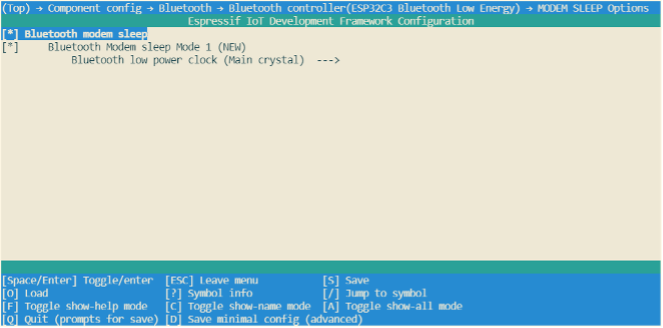
\includegraphics[width=0.9\textwidth]{D12Z/12-1}
    \caption{Modem-sleep mode of ESP32-C3 Bluetooth LE}
\end{figure}

\subsection{Light-sleep Mode}
Light-sleep mode functions in a similar manner to Modem-sleep mode, with the exception that in Light-sleep mode, the ESP32-C3 will power down the RF module and digital peripherals, while most of the RAM will be limited by clock gating. Additionally, the CPU will be paused, resulting in lower power consumption compared to Modem-sleep mode. After waking up from Light-sleep mode, ESP32-C3's peripherals and CPU will resume operation, and their internal state will be preserved. The wakeup latency in Light-sleep mode is less than 1 ms. There are two ways to put ESP32-C3 into Light-sleep mode:

\begin{term}{Entering Light-sleep mode manually}
    This is achieved by calling APIs. To enter Light-sleep mode manually, it is necessary to configure Wi-Fi as a wakeup source to allow the device to receive interactive information from either a smartphone or a server through the router.
\end{term}

\begin{term}{Entering Light-sleep mode automatically}
    After being configured to automatically enter Light-sleep mode, ESP32-C3 will automatically enter Light-sleep mode when the CPU and RF module are idle and can be automatically woken up to receive interactive information from the smartphone or server through the router.
\end{term}

\textbf{1. Wakeup sources in Light-sleep mode}

Manually entering Light-sleep mode requires configuring a wakeup source, which can be set to timers, GPIOs, UART, Wi-Fi, or Bluetooth LE for ESP32-C3. ESP32-C3 supports configuring one or more wakeup sources at the same time, in which case ESP32-C3 will be woken up when either wakeup source is triggered. Users can use \verb|esp_sleep_enable_*_wakeup()| function to configure wakeup sources, or use \verb|esp_sleep_disable_wakeup_source()| function to disable a wakeup source. Before entering Light-sleep mode, users can configure the wake source at any time. After waking up, users can determine which wakeup source was responsible for waking up the chip by calling \verb|esp_sleep_get_wakeup_cause()| function. Available wakeup sources in Light-sleep include:

\begin{term}{GPIO wakeup}
    Any GPIO can be used as the external input to wake up the chip from Light-sleep mode. Each pin can be individually configured to trigger wakeup on high or low level using the \verb|gpio_wakeup_enable()| function. GPIO wakeup can be used for any type of GPIO (RTC IO or digital IO). Then the \verb|esp_sleep_enable_gpio_wakeup()| function should be called to enable this wakeup source.
\end{term}

\begin{term}{Timer wakeup}
    The RTC controller has a built-in timer which can be used to wake up the chip after a predefined amount of time. Time is specified at microsecond precision, but the actual resolution depends on the clock source selected for the RTC \verb|SLOW_CLK|. RTC peripherals or RTC memories don’t need to be powered on during sleep in this wakeup mode. \verb|esp_sleep_enable_ timer_wakeup()| function can be used to enable sleep wakeup using a timer.
\end{term}

\begin{term}{UART wakeup}
    When ESP32-C3 receives UART input from external devices, it is often necessary to wake up the chip when input data is available. The UART peripheral contains a feature which allows waking up the chip from Light-sleep mode when a certain number of rising edges on RX pin are seen. This number of rising edges can be set using \verb|uart_set_wakeup_thre|\\ \verb|shold()|. Note that the character which triggers wakeup (and any characters before it) will not be received by the UART after wakeup. This means that the external device typically needs to send an extra character to the ESP32-C3 to trigger wakeup before sending the data. \verb|esp_sleep_enable_uart_wakeup()| function can be used to enable this wakeup source.
\end{term}

\begin{term}{Wi-Fi wakeup}
    When maintaining a Wi-Fi connection is required, the Wi-Fi can be configured as a wake source to wake up ESP32-C3. The ESP32-C3 wakes up before each DTIM beacon of the AP arrives and turns on its RF module, thus maintaining a Wi-Fi connection. \verb|esp_sleep_en|\\ \verb|able_wifi_wakeup()| function can be used to enable this wakeup source.
\end{term}

\textbf{2. Entering Light-sleep mode manually}

To manually enter the Light-sleep mode, users can call corresponding APIs to send ESP32-C3 into Light-sleep mode when needed. After entering Light-sleep mode, ESP32-C3 will turn off the RF module and pause its CPU. After waking up from Light-sleep mode, ESP32-C3 will continue to execute the original program at the location where the Light-sleep API was called. After manually entering the Light-sleep mode, ESP32-C3 can maintain the connection to the router by enabling Wi-Fi as the wake source and receive interactive information from the smartphone or server through the router. However, if Wi-Fi is not enabled as a wake source, ESP32-C3 may not receive packets in the network or disconnect the Wi-Fi connection. The situation of enabling/disabling Bluetooth LE as a wake source is similar.

\note{
\textbullet\ After calling the interface that manually send the chip into Light-sleep mode, ESP32-C3 will not immediately enter the Light-sleep mode, but will wait until the system is idle first.

\leftskip 1em
\textbullet\ With the Wi-Fi wakeup source enabled, only by entering the Light-sleep mode manually can ESP32-C3 maintain the connection with the router and receive the data sent in the network.}

\textbf{3. Instructions on how to enter Light-sleep mode manually}

After configuring the wakeup source, users can manually send the chip into Light-sleep mode by calling \verb|esp_light_sleep_start()| function. The code is as follows:

\begin{codebloc}
\begin{tabular}{d}
\vspace{2pt}
\begin{verbatim}
1.  #define BUTTON_WAKEUP_LEVEL_DEFAULT 0
2.  #define BUTTON_GPIO_NUM_DEFAULT     9
3.
4.  /*Configure the button GPIO as input, enable wakeup*/
5.  const int button_gpio_num   = BUTTON_GPIO_NUM_DEFAULT;
6.  const int wakeup_level      = BUTTON_WAKEUP_LEVEL_DEFAULT;
7.  gpio_config_t config = {
8.          .pin_bit_mask   = BIT64(button_gpio_num),
9.          .mode           = GPIO_MODE_INPUT
10. };
11. ESP_ERROR_CHECK(gpio_config(&config));
12. gpio_wakeup_enable(button_gpio_num, wakeup_level == 0 ?
13.                    GPIO_INTR_LOW_LEVEL : GPIO_INTR_HIGH_LEVEL);
14.
\end{verbatim}
\verb|15. /*Wake up in 2 seconds, or when button is pressed*/|
\end{tabular}
\end{codebloc}

\begin{codebloc}
\begin{tabular}{d}
\vspace{2pt}
\begin{verbatim}
16. esp_sleep_enable_timer_wakeup(2000000);
17. esp_sleep_enable_gpio_wakeup();
18.
19. /*Enter sleep mode*/
20. esp_light_sleep_start();
\end{verbatim}
\verb|21. /*Execution continues here after wakeup*/|
\end{tabular}
\end{codebloc}

When no wakeup source is enabled, ESP32-C3 can still enter Light-sleep mode. However, in this case, ESP32-C3 will remain in Light-sleep mode until an external chip reset.

\textbf{4. Entering Light-sleep mode automatically}

ESP32-C3 can be configured to automatically enter Light-sleep mode when it is idle and does not need the RF module to work, and automatically woken up when it needs to work (such as maintaining Wi-Fi and Bluetooth LE connections or receiving data). In this case, users don’t need to send the chip into Light-sleep mode manually, nor configure the wakeup source separately. After being configured to automatically enter Light-sleep mode, ESP32-C3 can maintain the connection to the router and receive interactive information from the smartphone or server through the router, thus improving user experience. The Bluetooth LE connection is similar to connecting to a router. Typically, automatic Light-sleep mode is used in conjunction with Modem-sleep mode and power management. When its RF module is not required, ESP32-C3 first enters Modem-sleep mode. If it is idle at this time, ESP32-C3 will enter Light-sleep mode to further reduce power consumption. The Modem-sleep mode of ESP32-C3 is shown in Figure 12.2.

\begin{figure}[!h]
    \centering
    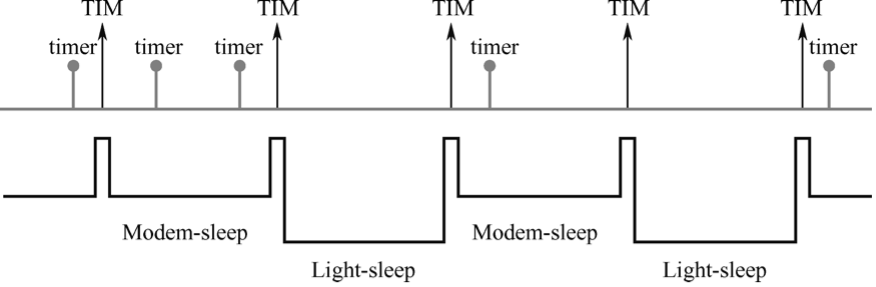
\includegraphics[width=0.8\textwidth]{D12Z/12-2}
    \caption{Modem-sleep mode of ESP32-C3}
\end{figure}

Automatic Light-sleep mode can be useful in scenarios that require ESP32-C3 to maintain a connection with the router and respond to data sent by the router in real time, but can be idle when no data needs to be received. For example, in the application of a Wi-Fi smart switch, the CPU remains idle most of the time until it receives a control command. Only upon receiving this command, the CPU activates and controls the switch to turn on or off.

\textbf{5. Instructions on how to enter Light-sleep mode automatically}

To configure enable the automatic Light-sleep mode, users can call \verb|esp_pm_configure()| function and set parameter \verb|light_sleep_enable| to \verb|true|. When this feature is enabled, note that \verb|CONFIG_FREERTOS_USE_TICKLESS_IDLE| and \verb|CONFIG_PM_ENABLE| options must also be configured.

To configure \verb|CONFIG_PM_ENABLE| option, users can run \verb|idf.py menuconfig| command to start the configuration tool, go to \verb|Component config| → \verb|Power Management|, then enable \verb|Support for power management|. The configuration of the ESP32-C3 power management function is shown in Figure 12.3.

\begin{figure}[!h]
    \centering
    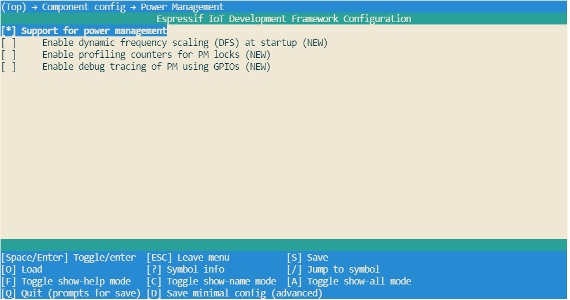
\includegraphics[width=0.85\textwidth]{D12Z/12-3}
    \caption{ESP32-C3 power management configuration}
\end{figure}

Users can enable the Dynamic Frequency Modulation (DFS) feature and configure the chip to automatically enter Light-sleep mode by calling \verb|esp_pm_configure()| function. When using ESP32-C3, the corresponding parameter of this function is \verb|esp_pm_config_esp32|\\ \verb|c3_t|, which is a structure that defines the relevant DFS settings and controls if the chip can automatically enter Light-sleep mode. In the above structure, the following three member variables (fields) need to be initialised:

\begin{itemize}[leftmargin=1em]
    \item \verb|max_freq_mhz|: Maximum CPU frequency in MHz, i.e., the frequency used when \verb|ESP_|\\ \verb|PM_CPU_FREQ_MAX| lock is acquired. This field is usually set to \verb|CONFIG_ESP32C3_|\\ \verb|DEFAULT_CPU_FREQ_MHZ|.
    \item \verb|min_freq_mhz|: Minimum CPU frequency in MHz, i.e., the frequency used when only the \verb|ESP_PM_APB_FREQ_MAX| lock is acquired. This field can be set to the XTAL frequency value, or the XTAL frequency divided by an integer. Note that 10 MHz is the lowest frequency at which the default \verb|REF_TICK| clock of 1 MHz can be generated.
    \item \verb|light_sleep_enable|: Whether ESP32-C3 should automatically enter Light-sleep mode when no locks are acquired (\verb|true|/\verb|false|).
\end{itemize}

Automatic Light-sleep mode is based on FreeRTOS Tickless Idle functionality. If Automatic Light-sleep mode is requested while the option \verb|CONFIG_FREERTOS_USE_TICKLESS_IDLE| is not enabled in \verb|menuconfig|, \verb|esp_pm_configure()| will return the error \verb|ESP_ERR_|\\ \verb|NOT_SUPPORTED|. Configuration of ESP32-C3’s FreeRTOS Tickless Idle feature is shown in Figure 12.4.

\begin{figure}[!h]
    \centering
    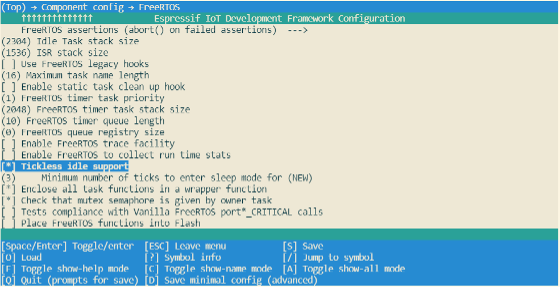
\includegraphics[width=0.9\textwidth]{D12Z/12-4}
    \caption{Configuration of ESP32-C3’s FreeRTOS Tickless Idle feature}
\end{figure}

\begin{codebloc}
\begin{tabular}{d}
\vspace{2pt}
\begin{verbatim}
1.  #if CONFIG_PM_ENABLE
2.      Configure dynamic frequency scaling:
3.      automatic light sleep is enabled if tickless idle support is enabled.
4.      esp_pm_config_ESP32-C3_t pm_config = {
5.          .max_freq_mhz = 160, //Maximum CPU frequency
6.          .min_freq_mhz = 10,  //Minimum CPU frequency
7.  #if CONFIG_FREERTOS_USE_TICKLESS_IDLE
8.          .light_sleep_enable = true
9.  #endif
10.         };
11.         ESP_ERROR_CHECK( esp_pm_configure(&pm_config) );
\end{verbatim}
\verb|12. #endif //CONFIG_PM_ENABLE|
\end{tabular}
\end{codebloc}

\subsection{Deep-sleep mode}
Compared to Light-sleep mode, ESP32-C3 cannot automatically enter Deep-sleep mode. Instead, users must call \verb|esp_deep_sleep_start()| function to send the chip into Deep-sleep mode. In Deep-sleep mode, ESP32-C3 does not maintain Wi-Fi and Bluetooth LE connections, and shuts down the CPU, most of the RAM and all digital peripherals clocked by the APB\_CLK. However, RTC clock controllers, RTC peripherals, and RTC fast memory can still work. After waking up from Deep-sleep mode, ESP32-C3’s CPU will reset and restart.

Deep-sleep can be used for low-power sensor applications, or application scenarios where data transmission is not required for most of the time. ESP32-C3 can wake up from Deep-sleep mode every once in a while to measure and upload data, after which it returns to Deep-sleep mode. Alternatively, the chip can also store data from multiple measurements in RTC Memory (RTC Memory can still save data in Deep-sleep mode) and send the data out at once.

\textbf{1. Wakeup sources in Deep-sleep mode}

For Deep-sleep mode, ESP32-C3 can use GPIO or timer as wakeup sources and supports up to two wakeup sources at the same time. In this case, ESP32-C3 will be woken up when either of the wakeup sources is triggered. Before entering Deep-sleep mode, users can either configure the wake source at any time using the corresponding API or disable a wake source using \verb|esp_sleep_ disable_wakeup_source()| function. After waking up, users can determine which wakeup source was responsible for waking up the chip by calling \verb|esp_sleep_get_wakeup_cause()| function.

\begin{term}{GPIO wakeup}
    Any GPIO can be used as the external input to wake up the chip from Deep-sleep mode. Each pin can be individually configured to trigger wakeup on high or low level using \verb|esp_deep_sleep_enable_gpio_wakeup()| function. It is important to note that GPIO wakeup is only available for RTC IO.
\end{term}

\begin{term}{Timer wakeup}
    The RTC controller has a built-in timer which can be used to wake up the chip after a predefined amount of time. Time is specified at microsecond precision, but the actual resolution depends on the clock source selected for \verb|RTC_SLOW_CLK|. When Timer wakeup is enabled, RTC peripherals or RTC memory do not need to be turned on during ESP32-C3 sleep, and Timer wakeup can be enabled by calling \verb|esp_sleep_enable_timer_wake| \verb|up()|.
\end{term}

\textbf{2. Instructions on how to enter Deep-sleep mode}

After configuring the wakeup source, users can call \verb|esp_deep_sleep_start()| to enter Deep-sleep mode. When no wakeup source is enabled, ESP32-C3 can still enter Deep-sleep mode. However, in this case, ESP32-C3 will remain in Deep-sleep mode until an external chip reset.

The following code shows how to configure ESP32-C3’s Deep-sleep mode.

\begin{itemize}
    \item Wakeup source: GPIO and timer;
    \item GPIO4 pin is configured to wake up on high level;
    \item The predefined amount of time to wake up the chip using a timer is 20 seconds. 
\end{itemize}

Considering that the GPIO4 pin wakes up ESP32-C3 at a high level, it is necessary to add a pull-down resistor in your hardware circuits or software configuration to avoid false wakeup.

\begin{codebloc}
\begin{tabular}{d}
\vspace{2pt}
\begin{verbatim}
1.  #define DEFAULT_WAKEUP_PIN    4
2.  #define DEFAULT_WAKEUP_LEVEL  ESP_GPIO_WAKEUP_GPIO_HIGH
3.  
4.  const gpio_config_t config = {
5.      .pin_bit_mask = BIT(DEFAULT_WAKEUP_PIN),
6.      .mode           = GPIO_MODE_INPUT,
7.  };
8.  ESP_ERROR_CHECK(gpio_config(&config));
9.  ESP_ERROR_CHECK(esp_deep_sleep_enable_gpio_wakeup(BIT(DEFAULT_WAKEUP_PIN),
10.                 DEFAULT_WAKEUP_LEVEL));
11. ESP_LOGI("TAG", "Enabling GPIO wakeup on pins GPIO%d\n",
12.          DEFAULT_WAKEUP_PIN);
13.
14. const int wakeup_time_sec = 20;
15. ESP_LOGI("TAG", "Enabling timer wakeup, %ds\n", wakeup_time_sec);
16. esp_sleep_enable_timer_wakeup(wakeup_time_sec * 1000000);
17.
18. /*Enter deep sleep*/
\end{verbatim}
\verb|19. esp_deep_sleep_start();|
\end{tabular}
\end{codebloc}

\subsection{Current Consumption in Different Power Modes}
The current consumption measurements are taken with a 3.3V supply at 25°C of ambient temperature at the RF port. All transmitters’ measurements are based on a 100\% duty cycle.

The current consumption depending on RF Modes is shown in Table 12.3.

\begin{table}[h!]
    \renewcommand{\arraystretch}{1.5}
    \caption{Current consumption depending on RF modes}
    \begin{NiceTabular}{|>{\Centering}m{9em}|>{\Centering}m{4em}|m{18em}|>{\Centering}m{5.5em}|}[hvlines]
    \CodeBefore
       \rowcolor{LightBlue}{1}
    \Body
    \textbf{Work mode}&\Block{1-2}{\textbf{Description}}&&\textbf{Peak (mA)}\\
    \Block{6-1}{Active (RF working)}&\Block{4-1}{TX}&IEEE 802.11b, 1 Mbit/s, @21dBm&335\\
    &&IEEE 802.11g, 54 Mbit/s, @19 dBm&285\\
    &&IEEE 802.11n, HT20, MCS7, @18.5 dBm&276\\
    &&IEEE 802.11n, HT40, MCS7, @18.5 dBm&278\\
    &\Block{2-1}{RX}&IEEE 802.11b/g/n, HT20&84\\
    &&IEEE 802.11n, HT20&87\\
    \end{NiceTabular}
\end{table}

Current consumption in other modes is shown in Table 12.4.

\begin{table}[h!]
    \renewcommand{\arraystretch}{1.4}
    \caption{Current consumption in other modes}
    \begin{NiceTabular}{|>{\Centering}m{8em}|>{\Centering}m{8em}|>{\Centering}m{8em}|>{\Centering}m{6em}|>{\Centering}m{6em}|}[hvlines]
    \CodeBefore
       \rowcolor{LightBlue}{1}
    \Body
    \textbf{Work mode}&\Block{1-2}{\textbf{Description}}&&\textbf{Typical value}&\textbf{Unit}\\
    \Block{2-1}{Modem-sleep$^{1,2}$}&\Block{2-1}{CPU working$^3$}&160 MHz&20&mA\\
    &&80 MHz&15&mA\\
    Light-sleep&\Block{1-2}{—}&&130&$\mu$A\\
    Deep-sleep&\Block{1-2}{RTC timer + RTC memory}&&5&$\mu$A\\
    Power off&\Block{1-2}{CHIP\_EN set to low level;\\chip being powered off}&&1&$\mu$A\\
    \end{NiceTabular}
\end{table}

\textbf{Table notes:}

\begin{enumerate}[label=$^\arabic*$]
    \item When measuring the power consumption of Modem-sloop mode, the CPU is running and the Cache is idle.
    \item In the scenario when Wi-Fi is enabled, the chip switches between Active mode and Modem-sleep mode, and the current consumption will also change between the two modes.
    \item In Modem-sleep mode, the CPU frequency changes automatically, and the frequency depends on the CPU load and the peripherals used.
\end{enumerate}

\section{Power Management and Low-Power Debugging}
Please note that the actual power consumption may exceed theoretical values due to various factors, such as but not limited to:

\begin{itemize}
    \item Wi-Fi is receiving data or Bluetooth LE is receiving data.
    \item The application acquires the power management lock for a long time and does not release it.
    \item Process blocking (that is not related to calling operating system APIs) exists in the application.
    \item The predefined interval to wake up the chip via a timer is too small or interrupts happen too often.
\end{itemize}

It’s advised to identify the root cause and seek optimisation if the power consumption exceeds theoretical values for a substantial amount of time. Users can identify the root cause via log debugging and GPIO debugging, or additionally use some network protocol analysers if the high-power consumption may relate to Wi-Fi and Bluetooth LE. Note that this process can iterate as many times as needed till the actual product requirements are met.

The following sections describe the most commonly used methods to optimise power consumption, namely log debugging and GPIO debugging, and demonstrate how to put these methods into practice through real-world examples and real-time power consumption data.

\subsection{Log Debugging}
When using the log debugging feature, users need to configure \verb|CONFIG_PM_PROFILING| in \verb|menuconfig| to track the retention time of each power management lock, then call \verb|esp_pm_dump_locks (FILE* stream)| function to print such log. Log debugging allows users to analyse which power management locks are preventing the chip from entering a low-power mode and check how much time the chip spends in each power mode. After debugging, users must disable \verb|CONFIG_PM_PROFILING| in \verb|menuconfig|.

To configure \verb|CONFIG_PM_PROFILING|, users need to run \verb|idf.py menuconfig| command to start the configuration tool, go to \verb|Component config| → \verb|Power Management|, and enable \verb|Enable profiling counters for PM locks|. The screenshot of how to enable the log debugging for ESP32-C3 is shown in Figure 12.5.

\begin{figure}[!h]
    \centering
    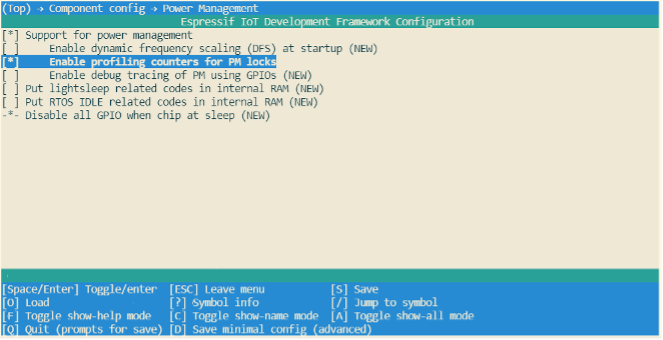
\includegraphics[width=0.9\textwidth]{D12Z/12-5}
    \caption{Configuration of ESP32-C3’s low-power log debugging}
\end{figure}

When ESP32-C3 is configured to automatically enter Light-sleep mode, users must call \verb|esp_pm_dump_locks (FILE* stream)| function periodically to print debugging log and analyse the root cause of increased power consumption. Some log debugging information is provided below:

\begin{codebloc}
\begin{tabular}{d}
\vspace{2pt}
\begin{verbatim}
Time: 11879660
Lock stats:
name              type            arg  cnt     times      time      percentage
wifi              APB_FREQ_MAX    0    0        107       1826662   16%
bt                APB_FREQ_MAX    0    1        126       5367607   46%
rtos0             CPU_FREQ_MAX    0    1       8185       809685    7%
Mode stats:
name     HZ        time     percentage
SLEEP     40M      4252037  35%
APB_MIN   40M            0   0%
APB_MAX   80M      6303881  53%
\end{verbatim}
\verb|CPU_MAX  160M       823595   6%|
\end{tabular}
\end{codebloc}

The \verb|esp_pm_dump_locks (FILE* stream)| function prints two types of debugging information, namely the \verb|Lock stats| and \verb|Mode stats|. The Lock stats section lists the real-time status of all power management locks used by the application with the following information: Name (\verb|name|), type of power management lock (\verb|type|), parameter (\verb|arg|), number of times the power management lock is currently acquired (\verb|cnt|), total number of times the power management lock is acquired (\verb|times|), total amount of time the power management lock is acquired (\verb|time|), and the proportion of time when the power management lock is acquired (\verb|percentage|). The Mode stats section lists the real-time status of the application’s different modes with the following information: Mode name (\verb|name|), clock frequency (\verb|HZ|), total amount of time in the mode (\verb|time|), and percentage of the amount of time in the mode (\verb|percentage|).

By checking the example log above, users can easily find out that, for the \verb|Wi-Fi| power management lock \verb|APB_FREQ_MAX|, 

\begin{itemize}
    \parskip 0pt
    \item this lock is currently not acquired,
    \item the total amount time when this lock was acquired is 1826662 $\mu$s,
    \item the total number of this lock being acquired is 107 times,
    \item and the proportion of time when this lock was acquired is 16\%. 
\end{itemize}

Similarly, users can also know the \verb|rtos0| power management lock \verb|CPU_FREQ_MAX|:

\begin{itemize}
    \parskip 0pt
    \item is currently being acquired,
    \item the total amount time when this lock was acquired is 809685 $\mu$s,
    \item the total number of this lock being acquired is 8185 times,
    \item and the proportion of time when this lock was acquired is 7\%.
\end{itemize}

Also, users can read log information about the Mode stats in a similar way. For example, in Sleep mode the clock frequency is 40 MHz, and the total time in this mode is 4252037 $\mu$s, accounting for 35\% of the whole time. Similarly, users can read the log for other locks and states themselves.

\subsection{GPIO Debugging}
When using GPIO debugging, users need to go to \verb|menuconfig|, and enable \verb|CONFIG_PM_| \verb|TRACE|. If enabled, some GPIOs will be used to signal events such as RTOS ticks, frequency switching, entry/exit from idle state. For a list of GPIOs, see \verb|pm_trace.c| file. This feature is intended to be used when analysing/debugging behavior of power management implementation and should be kept disabled after the debugging.

The relevant GPIOs are shown below, with two GPIOs for each event, corresponding to CPU0 and CPU1. Since ESP32-C3 is a single-core chip, only the first column of GPIOs is effective when debugging. During development, users can also modify the GPIO used by modifying the source code. Before debugging, connect the selected GPIO to an instrument such as a logic analyser or oscilloscope.

\begin{codebloc}
\begin{tabular}{d}
\vspace{2pt}
\begin{verbatim}
1.	/*GPIOs to use for tracing of esp_pm events.
2.	* Two entries in the array for each type, one for each CPU.
3.	* Feel free to change when debugging.
4.	*/
5.	static const int DRAM_ATTR s_trace_io[] = {
6.	#ifndef CONFIG_IDF_TARGET_ESP32C3
7. 	    BIT(4),  BIT(5),  		//ESP_PM_TRACE_IDLE
8. 	    BIT(16), BIT(17), 		//ESP_PM_TRACE_TICK
9. 	    BIT(18), BIT(18), 		//ESP_PM_TRACE_FREQ_SWITCH
10.     BIT(19), BIT(19), 		//ESP_PM_TRACE_CCOMPARE_UPDATE
11.     BIT(25), BIT(26), 		//ESP_PM_TRACE_ISR_HOOK
12.     BIT(27), BIT(27), 		//ESP_PM_TRACE_SLEEP
13.	#else
14.     BIT(2),  BIT(3),  		//ESP_PM_TRACE_IDLE
15.     BIT(4),  BIT(5),  		//ESP_PM_TRACE_TICK
16.     BIT(6),  BIT(6),  		//ESP_PM_TRACE_FREQ_SWITCH
17.     BIT(7),  BIT(7),  		//ESP_PM_TRACE_CCOMPARE_UPDATE
18.     BIT(8),  BIT(9),  		//ESP_PM_TRACE_ISR_HOOK
19.     BIT(18), BIT(18), 		//ESP_PM_TRACE_SLEEP
20.	#endif
\end{verbatim}
\verb|21.	};|
\end{tabular}
\end{codebloc}

To enable \verb|CONFIG_PM_PROFILING|, users need to run the \verb|idf.py menuconfig| command to start the configuration tool, go to \verb|Component config| → \verb|Power Management|, and enable \verb|Enable debug tracing of PM using GPIOs|. The screenshot of how to Enable debug tracing of PM using GPIOs for ESP32-C3 is shown in Figure 12.6.

\begin{figure}[!h]
    \centering
    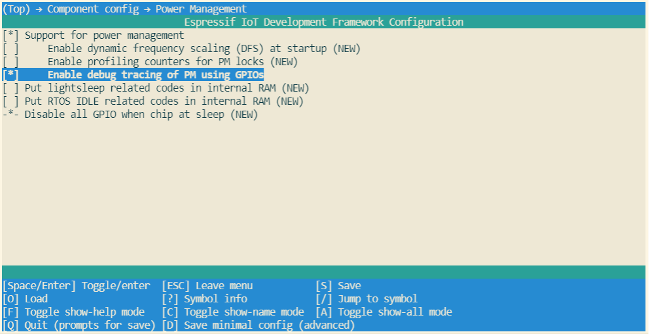
\includegraphics[width=0.85\textwidth]{D12Z/12-6}
    \caption{ESP32-C3 low-power GPIO debug configuration}
\end{figure}

The debugging can begin after completing the above-mentioned configuration. By observing different GPIO states, users get to know the current state of the CPU and the corresponding power mode, and further understand which power modes consume more power and can be optimised. Figure 12.7 shows the waveform of ESP32-C3’s GPIO debugging for reduced power consumption. The upper section shows the real-time power consumption of ESP32-C3, and the lower section shows the GPIO waveform corresponding to \verb|ESP_PM_TRACE_SLEEP| event.

\begin{figure}[!h]
    \centering
    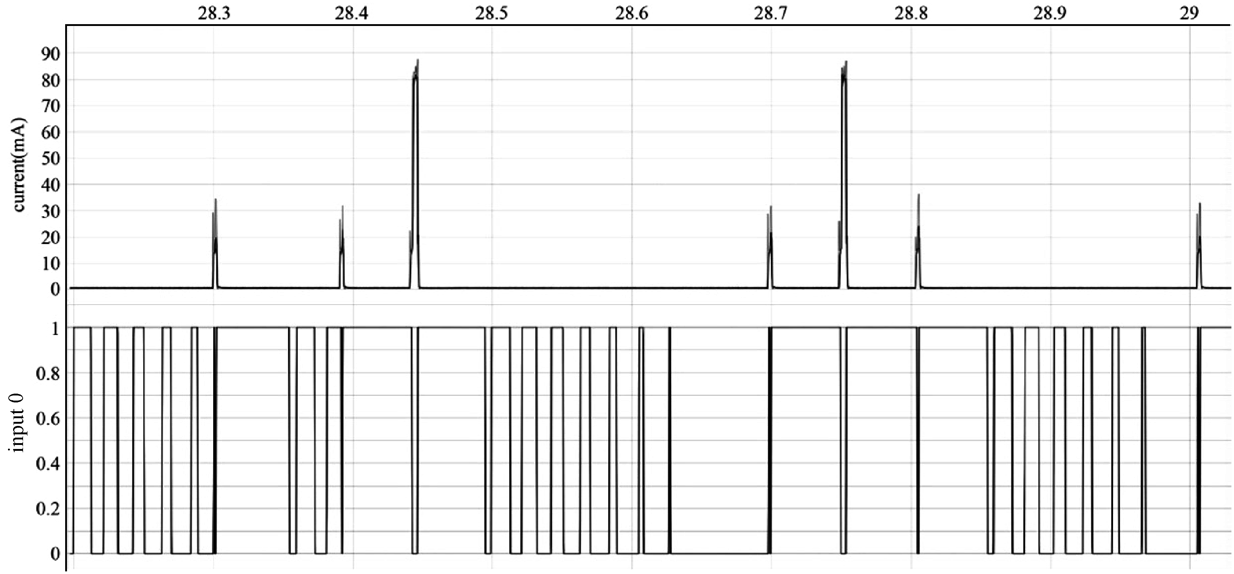
\includegraphics[width=0.85\textwidth]{D12Z/12-7}
    \caption{ESP32-C3 low-power GPIO debug waveform}
\end{figure}

\section{Practice: Power Management in Smart Light Project}
After understanding ESP32-C3’s power management feature and different low-power modes, users can implement different power management schemes to reduce power consumption during the development of their actual IoT projects. This section introduces how to optimise the power consumption of the Smart Light project, which is also used as an example in other sections of this book, by implementing ESP32-C3's power management scheme and using different low-power modes.

To save energy in general or obtain certification for energy consumption, it is necessary to reduce the power consumption of ESP32-C3 during operation as much as possible in the Smart Light project. As explained in Sections 12.1 and 12.2, when ESP32-C3 is operating in Deep-sleep mode, its LEDC function does not work properly, and its Wi-Fi and BLE connections cannot be maintained. As a result, ESP32-C3 can not receive control commands from the user. Therefore, a power management scheme that utilises Wi-Fi Modem-sleep mode, Bluetooth Low Energy Modem-sleep mode, power management, and automatic Light-sleep mode is commonly employed to minimise power consumption in smart light projects. After implementing this scheme:

\begin{itemize}[leftmargin=1.5em]
    \item When the light is on, the power management lock is acquireed to ensure that the LEDC works normally, while Wi-Fi and Bluetooth LE remain connected to receive the user's control commands. By using the Modem-sleep mode of Wi-Fi and the Modem-sleep mode of Bluetooth LE, the working time of the RF circuit can be reduced to reduce power consumption.
    \item When the light is off, the power management lock is released so CPU can enter Light-sleep mode when it is idle to further reduce power consumption.
\end{itemize}

Implementing this scheme in the Smart Light project involves two steps:

\begin{enumerate}[label=(\arabic*)]
    \item Configure ESP32-C3’s power management feature, enable Automatic Light-sleep mode, turn on Wi-Fi Modem-sleep mode and Bluetooth LE Modem-sleep mode.
    \item Complete the operation of the power management lock in the application so the driver for LEDC dimming works properly.
\end{enumerate}

To learn how to optimise for lower power consumption for your existing projects, please visit \href{https://github.com/espressif/book-esp32c3-iot-projects/tree/main/device_firmware/6_project_optimize}{\texttt{book-esp32c3-iot-projects/device\_firmware/6\_project\_optimize}}.

\subsection{Configuring Power Management Feature}
(1) Enabling the power management feature and Automatic Light-sleep mode.

When enabling the power management feature, users first need to enable the corresponding options in \verb|menuconfig|, then call \verb|esp_pm_configure()| function (Please select \verb|esp_pm_|\\ \verb|config_esp32c3_t| when you are developing with ESP32-C3). For instructions on how to enable the Automatic Light-sleep mode, please check Section 12.2.2.

(2) Configuring \verb|Wi-Fi Modem-sleep & Bluetooth Modem-sleep|.

\begin{itemize}
    \item To enable \verb|Bluetooth Modem-sleep mode|, just enable the option in \verb|menuconfig| shown in the screenshot below.
    \begin{figure}[!h]
        \centering
        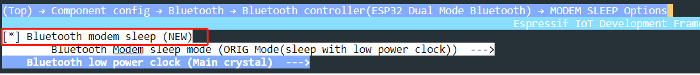
\includegraphics[width=0.95\textwidth]{D12Z/12-8}
        \caption{ESP32-C3’s \texttt{Bluetooth LE Modem-sleep} configuration}
    \end{figure}
    \item To enable Wi-Fi modem-sleep mode, users need to first initialise Wi-Fi, and then call \verb|esp_wifi_set_ps(wifi_ps_type_t type)| function. The code to enable Wi-Fi modem-sleep mode for the Smart Light project is as follows:
\end{itemize}

\begin{codebloc}
\begin{tabular}{d}
\vspace{2pt}
\begin{verbatim}
1.	#define LISTEN_INTERVAL 3
2.	wifi_config_t wifi_config = {
3. 	    .sta = {
4. 	        .ssid = "SSID",
5. 	        .password = "Password",
6. 	        .listen_interval = LISTEN_INTERVAL,
7. 	    },
8.	};
9.	ESP_ERROR_CHECK(esp_wifi_set_mode(WIFI_MODE_STA));
10. ESP_ERROR_CHECK(esp_wifi_set_config(ESP_IF_WIFI_STA, &wifi_config));
11. ESP_ERROR_CHECK(esp_wifi_start());
12.
\end{verbatim}
\verb|13. ESP_ERROR_CHECK(esp_wifi_set_ps(WIFI_PS_MAX_MODEM));|
\end{tabular}
\end{codebloc}

\subsection{Use Power Management Locks}
From Section 12.1.1, we understand when being clocked by clock sources except \verb|REF_TICK|, ESP32-C3’s LEDC is affected by dynamic FM, and code for acquiring/releasing the power management locks must be added in the application so the LEDC can function properly. Therefore, a power management lock is required in the application to ensure that the APB clock does not change while the LEDC is operating. Specifically: 

\begin{itemize}[leftmargin=1.5em]
    \item During the LEDC driver initialisation, initialise the \verb|ESP_PM_APB_FREQ_MAX| power management lock.
    \item When the LEDC starts working (light on), acquire the power management lock.
    \item And when the LEDC stops working (light off), release the power management lock. The code to enable Wi-Fi modem-sleep mode for the Smart Light project is as follows:
\end{itemize}

\begin{codebloc}
\begin{tabular}{d}
\vspace{2pt}
\begin{verbatim}
1.	static esp_pm_lock_handle_t s_pm_apb_lock   = NULL;
2.	
3.	if (s_pm_apb_lock == NULL) {
4. 	    if (esp_pm_lock_create(ESP_PM_APB_FREQ_MAX, 0, "l_apb",
5.                             &s_pm_apb_lock) ! = ESP_OK) {
6. 	        ESP_LOGE(TAG, "esp pm lock create failed");
7. 	    }
8.	}
9.	
\end{verbatim}
\verb|10. while (1) {|
\end{tabular}
\end{codebloc}

\begin{codebloc}
\begin{tabular}{d}
\vspace{2pt}
\begin{verbatim}
11.         ESP_ERROR_CHECK(esp_pm_lock_acquire(s_pm_apb_lock));
12.         ESP_LOGI(TAG, "light turn on");
13.         for (ch = 0; ch < LEDC_TEST_CH_NUM; ch++) {
14.             ledc_set_duty(ledc_channel[ch].speed_mode,
15.                           ledc_channel[ch].channel, LEDC_TEST_DUTY);
16.             ledc_update_duty(ledc_channel[ch].speed_mode,
17.                              ledc_channel[ch].channel);
18.         }
19.         vTaskDelay(pdMS_TO_TICKS(5 * 1000));
20.
21.         ESP_LOGI(TAG, "light turn off");
22.         for (ch = 0; ch < LEDC_TEST_CH_NUM; ch++) {
23.             ledc_set_duty(ledc_channel[ch].speed_mode,
24.                           ledc_channel[ch].channel, 0);
25.             ledc_update_duty(ledc_channel[ch].speed_mode,
26.                              ledc_channel[ch].channel);
27.         }
28.         ESP_ERROR_CHECK(esp_pm_lock_release(s_pm_apb_lock));
29.         vTaskDelay(pdMS_TO_TICKS(5 * 1000));
\end{verbatim}
\verb|30. }|
\end{tabular}
\end{codebloc}

\subsection{Verifying Power Consumption}
\begin{figure}[!h]
    \centering
    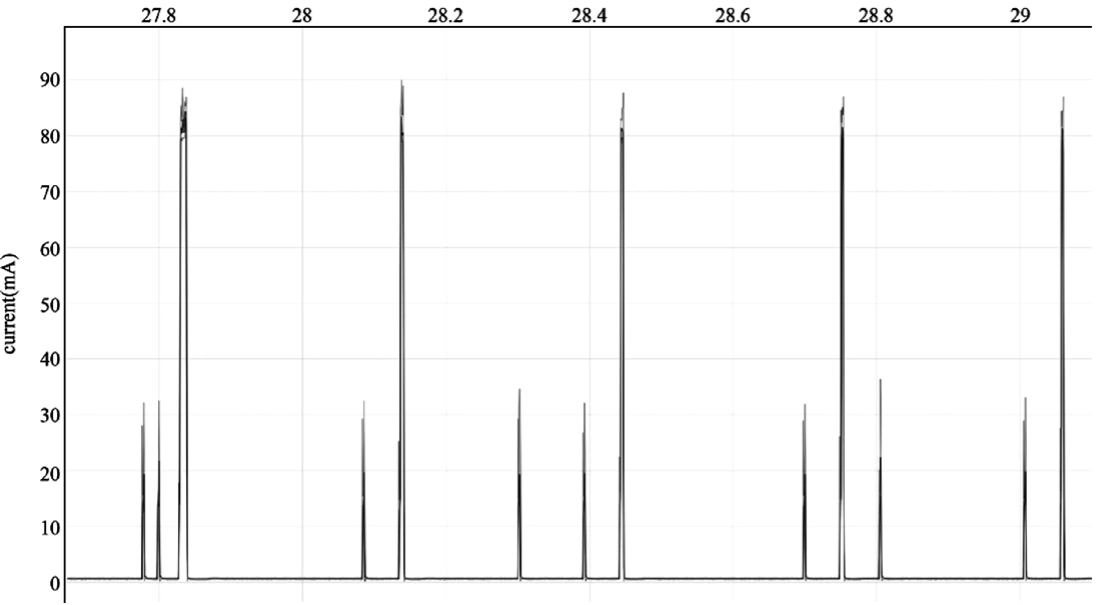
\includegraphics[width=0.8\textwidth]{D12Z/12-9}
    \caption{Average current of ESP32-C3 module}
\end{figure}
After completing all the above-mentioned configuration to reduce power consumption, it’s time to test the actual power consumption and check if it meets the power consumption requirements. According to the certification requirements, the actual DUT can be the whole light product or just the ESP32-C3 module. When the ESP32-C3 module is selected as the DUT, a power analyser can be added between the DC power supply and the chip to measure the power consumption data. The power analyser used in this book is Joulescope: Precision DC Energy Analyser. Among the certification requirements related to power consumption, it is often necessary for smart lighting devices to measure the average current when the lights are off and Wi-Fi is connected.

After implementing the power management scheme introduced above, the average current of the ESP32-C3 module is 2.24 mA (see Figure 12.9). Note that the actual test result may be different because Figure 12.9 only shows the power consumption of ESP32-C3 module for a short period of time.

\section{Summary}
In this chapter, we first introduced ESP32-C3’s power management feature and supported low-power modes (Modem-sleep, Light-sleep, Deep-sleep modes), then described how to perform low-power debugging, and, at last, concluded how to use the power management feature and low-power modes to reduce power consumption and how to measure actual power consumption, using a smart light project as an example.

\end{document}